\documentclass[fontsize=12pt]{scrartcl}

\usepackage[hyphens]{url}
\usepackage{hyperref}
\usepackage[pdftex]{graphicx}
\usepackage{listings}

\usepackage{sectsty}
\allsectionsfont{%
    \usefont{OT1}{bch}{b}{n}%
}

\sectionfont{%
	\usefont{OT1}{bch}{b}{n}%
	\sectionrule{0pt}{0pt}{-5pt}{0.8pt}%
}

\usepackage{fancyhdr}
\usepackage[margin=4.3cm]{geometry}
\pagestyle{fancyplain}

\title{ \vspace{-1in} 	\usefont{OT1}{bch}{b}{n}
    	\LARGE \strut \mbox{Translink~Magnetic~Stripe~Security}
 \vspace{-0.0in}
}

\author{ \usefont{OT1}{bch}{m}{n}
        Andrew Fuller\\		\usefont{OT1}{bch}{m}{n}
        Simon Fraser University\\
        \href{mailto:abf@sfu.ca}{\nolinkurl{abf@sfu.ca}}
}
\date{}

\begin{document}
\maketitle
 \vspace{-0.4in}
\section{Introduction}
In late 2001 Translink began replacing paper transit tickets with electronically-encoded magnetic tickets. These tickets are meant to counter fare evasion and ticket counterfeiting \cite{debut}. We found prior research which determined that these magnetic stripes contain data in an unknown format \cite{ubc}. In this report we decode this ticket format and create fully forged tickets using off-the-shelf hardware.

\begin{figure}[ht!]
\centering
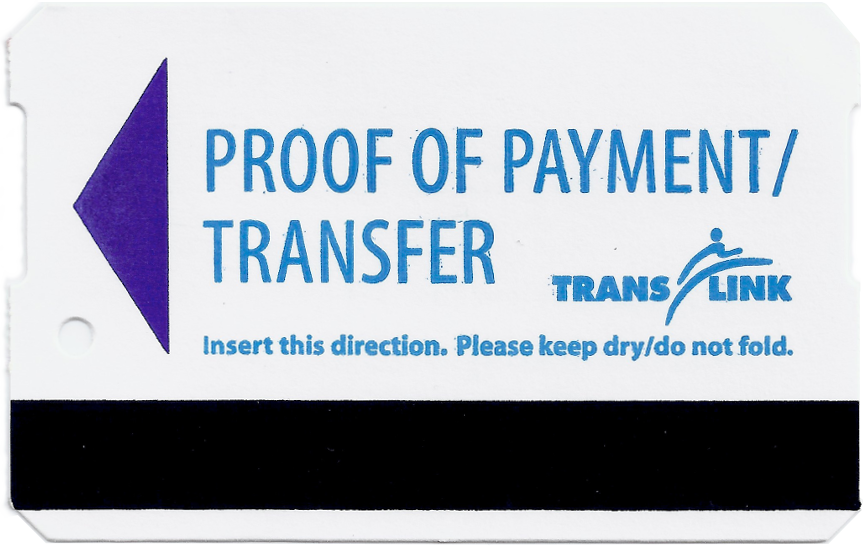
\includegraphics[width=90mm]{ticket1_front.png}
\caption{Translink magnetic stripe ticket}
\end{figure}

\section{Ticket collection}
We wanted to create a forged ticket without paying for any sample tickets for analysis. We spent several days in downtown Vancouver collecting used tickets from various locations. Eventually we managed to collect 45 tickets from the ground, and these were used for the initial analysis.

\section{Bit encoding}
In order to determine what kind of data are stored on the magnetic stripe, a small reader was built from a tape deck read head. We soldered the read head's signal wires to a 3.5mm stereo audio jack.

\begin{figure}[ht!]
\centering
\makebox[\textwidth]{

\includegraphics[width=30mm]{tape.png}
}
\caption{Tape read head}
\end{figure}

The stereo jack was plugged into a laptop's microphone input port, and the tape head was then be swiped along the magnetic stripe to create an audio waveform corresponding to the bit transitions encoded on the magnetic stripe. This waveform was displayed in Audacity for analysis, and it was determined that the bits were encoded using Aiken Biphase (F2M).

\begin{figure}[ht!]
\centering
\makebox[\textwidth]{
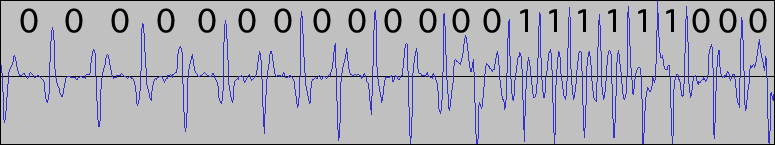
\includegraphics[width=100mm]{aiken_biphase_decoded.png}
}
\caption{Audacity waveform}
\end{figure}

We wrote a small program to automate the task of decoding the waveform into the resulting data bits. We then scanned the tickets that we had collected and entered the bit patterns into a spreadsheet for analysis.


\begin{figure}[ht!]
\centering
\makebox[\textwidth]{
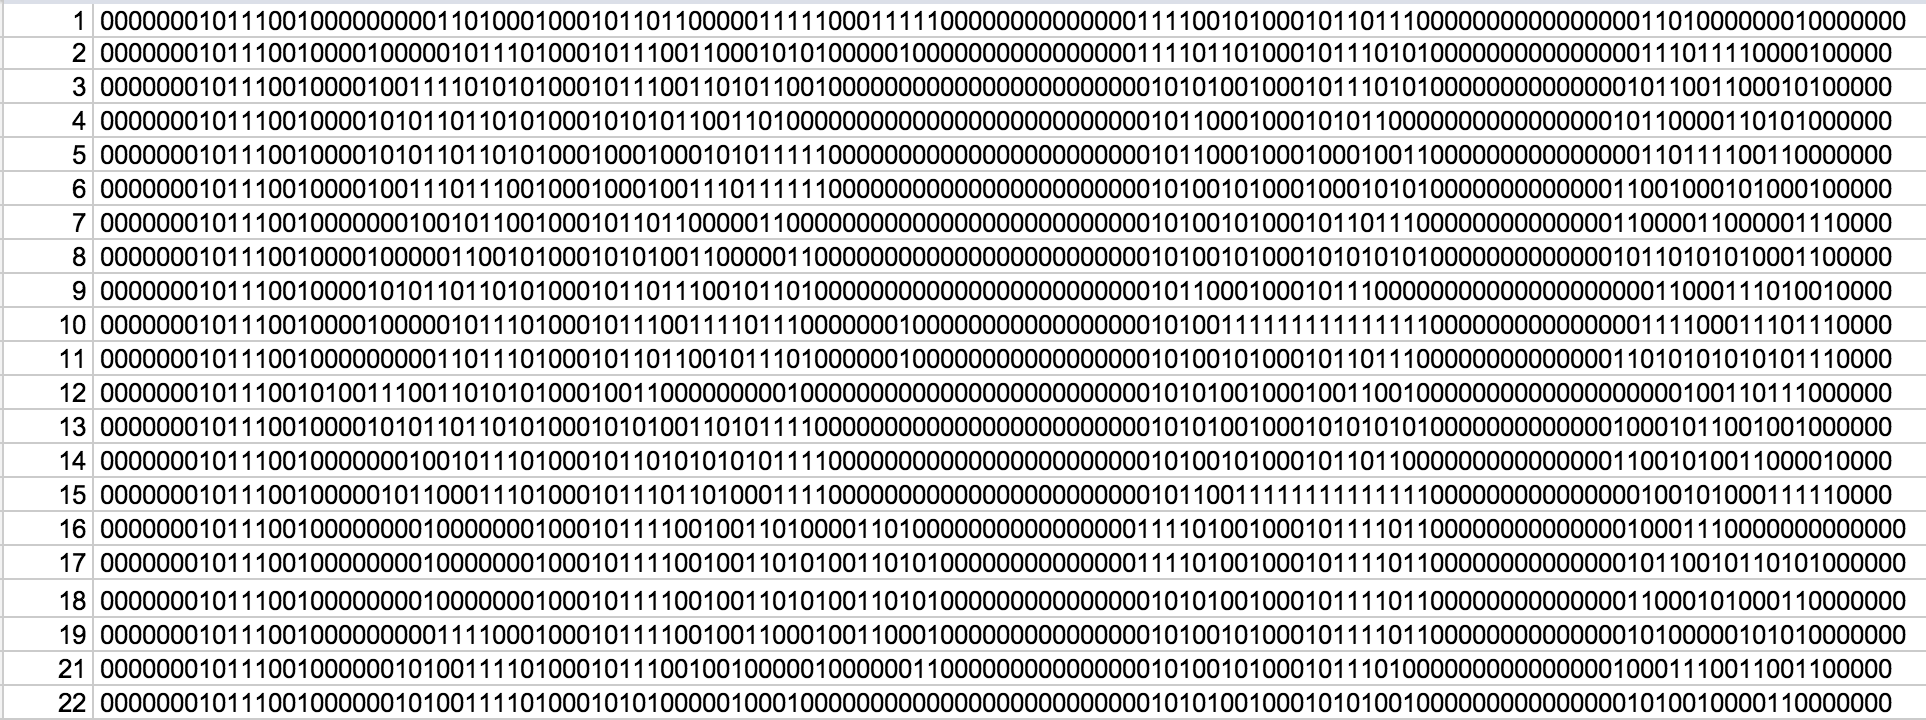
\includegraphics[width=140mm]{bits.png}
}
\caption{Ticket data}
\end{figure}

\section{Data format}
We began by looking for patterns in the bits that could represent dates or zone information. We knew that tickets always expire at times which are a multiple of 6 minutes (\texttt{:00}, \texttt{:06}, \texttt{:12} etc.) There are only $24 \times 10 = 240$ possible expiry times, which means this field can be stored in 8 bits. We eventually found several fields including ticket type (number of valid zones), ticket use (number of zones visited) and expiry time. We were limited by the small dataset, so we began collecting every ticket that we saw on the ground. By late March we had collected 800 tickets from various locations around Vancouver.

We collected samples of exotic ticket types such as Concession Daypass tickets and 3-zone faresavers. We also found old tickets that had fallen between seats and into the engine compartment of several buses. These new data allowed us to determine all of the data fields.
\\

\begin{tabular}{lll}
    Field no. & Length (bits) & Meaning \\
    1  & 1  & Blank ticket? \\
    2  & 32 & Serial number \\
    3  & 14 & Sign number \\
    4  & 14 & Expiry date \\
    5  & 8  & Expiry time \\
    6  & 8  & Flags \\
    7  & 1  & Daypass? \\
    8  & 1  & Concession? \\
    9  & 1  & Addfare? \\
    10 & 3  & Type \\
    11 & 2  & Value \\
    12 & 3  & Zones visited \\
    13 & 14 & Activation date \\
    14 & 16 & Checksum (FCS)
\end{tabular}
\\
\\

If the ticket is a Faresaver that has not been validated yet, then the first field will be a \texttt{1} bit and the following 32 bits contain the ticket's serial number (printed on the front of the ticket) as an unsigned integer. Upon use, Faresaver tickets will receive an Activation Date of 11111111111111, and this value is ignored by ticket machines.

Otherwise, the ticket has been validated and the expiry fields store the expiry date and time. The expiry date is stored as the number of days since December 31, 1999. The expiry time is stored as the number of 6-minute intervals since the previous 5:36PM. For example, a ticket which expires at 3:06AM on April 2, 2012 would have an expiry date field value of 4840 (01001011101000) and an expiry field value of 85 (01010101).

The ticket's value is stored as a 2-bit value representing the number of zones that can be visited (the value 00 is invalid). This information is duplicated in the 3-bit ticket type field, but that field is ignored by ticket reader machines.
\\

\begin{tabular}{ll}
Ticket type & Meaning \\
000 & ``Read error'' \\
001 & 1 Zone \\
010 & 2 Zone \\
011 & 3 Zone \\
100 & Concession 1 Zone \\
101 & Concession 2 Zone \\
110 & Concession 3 Zone / Addfare \\
111 & Daypass
\end{tabular}
\\
\\

The list of zones that a ticket has visited is stored in the Zones Visited field. Every transit vehicle records its current zone, and any new zones that the ticket visits will be recorded in the Zones Visited bitmask. This field is enforced by ticket reader software, so that a 2-zone ticket which has already visited 2 zones cannot be used in the third zone without a paid upgrade.

There are flag fields representing whether this ticket is a Concession ticket (for students), whether it is a Daypass, and whether it has had an Addfare applied to it. Note that when upgrading to an Addfare, ticket machines will dispose of the original ticket and print a new ticket with an updated value and the letter `A' beside it.

\section{Checksum}
As we scanned more and more tickets we could tell that the final 16 bits represented some kind of a security code or checksum. Identical tickets bought during the same 6-minute interval had the same bit sequence and the same checksum, and tickets whose bit sequence differed by only a single bit (same expiry time but different value) had radically different checksum fields.

We began by finding code to implement most well-known 16-bit checksum algorithms such as CRC-16, sum-16 and Fletcher-16. We collected a list of standard polynomials to use in several variants of CRC-16. However we weren't sure which bits were checksummed, and in what order. We then wrote software to apply every checksum variant to several of the ticket bit strings, trying every possible length and bit offset. After several days of computation a matching CRC was found: CRC-ITU (formerly CRC-CCITT). This uses a starting value of \texttt{0xffff} and a polynomial of \texttt{0x1021}.

We also determined that the Sign Number field produced identical values for a particular bus route. When a ticket is scanned at a new location, the Sign Number stored on the ticket is compared with the scanner's Sign Number. If the values don't match, the ticket is re-written with the current ticket machine's Sign Number. Using this knowledge we were almost ready to create a fully-forged ticket.

\section{Re-encoding}
We wrote a GUI program to facilitate the modification of ticket data. The program displays a virtual ticket on the screen, and when a ticket is swiped using the tape head, the signal is decoded using our Aiken-biphase decoder program, and the extracted field values are shown on the virtual ticket. These fields can be modified using the keyboard arrow keys, or typed in directly. The user can then hit Enter to produce the modified bitstring. We purchased an aftermarket copy of the Tyner MSR-206 credit card writer from Craigslist. This is a USB device which can encode and decode magnetic stripe data in Aiken-biphase format. However there were several problems that we encountered.



\begin{figure}[ht!]
\centering
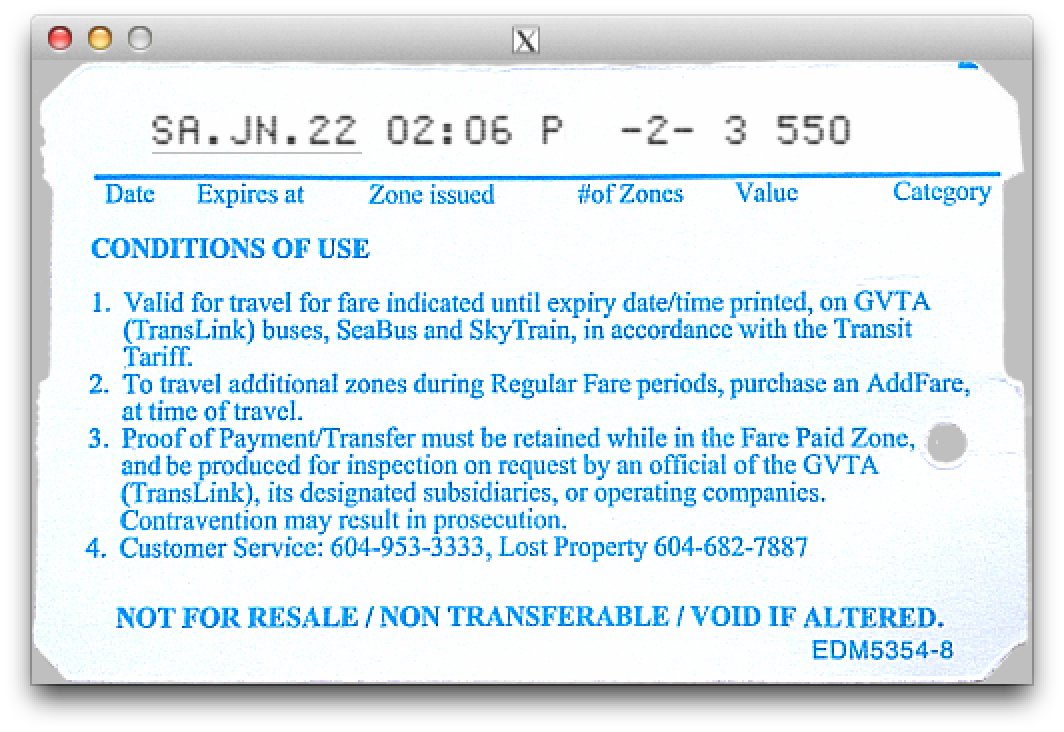
\includegraphics[width=130mm]{ss.png}
\caption{Screenshot of ticket modification GUI}
\end{figure}

The first problem is that the MSR-206 is used to write data to ISO standard magnetic stripe cards, and Translink magnetic tickets differ both in magnetic stripe position as well as ferrometallic composition. Credit card writers encode alphanumeric data in a specific format according to the magnetic track being used. We  reverse-engineered the write format used in the MSR-206 in order to write arbitrary bit sequences. The MSR-206 outputs approximately 50 leading `0' bits before the encoded data, but Translink tickets contain exactly 7 leading `0' bits. We taped a piece of magnetic stripe onto the left edge of a Translink ticket, so that the majority of the leading `0' bits would be written onto this scrap paper, absorbing most of the MSR-206's preamble and leaving  5-9 bits.

The bit density of Translink tickets is 80 bits/inch, which does not match the available write densities provided by the MSR-206 (75bpi and 210bpi) \cite{tyner}. However if the card is swiped at a slow speed, the MSR-206 will unintentionally write the data at a higher bpi.

The second problem is that the Translink ticket machines encode the data at an unusual position on the ticket. We created a support mechanism to allow us to precisely position the tape head as it was scanned across a sample ticket. This allowed us to create a high-resolution profile of where the data were located on the magnetic stripe. We determined that the data were stored exactly halfway between ISO track 1 and 2, approximately 8.5mm from the bottom edge of the ticket. We built a plastic harness to hold the ticket in a raised position, and use the MSR-206's track 1 write head to write the data at the appropriate location.

The resulting tickets appeared valid according to our analysis, but produced errors when scanned on Translink bus ticket readers. After several weeks of attempts, we discovered that the ticket validators at Burrard skytrain station are very old, and these machines have larger read heads that scan a larger track area for magnetic data.

\begin{figure}[ht!]
\centering
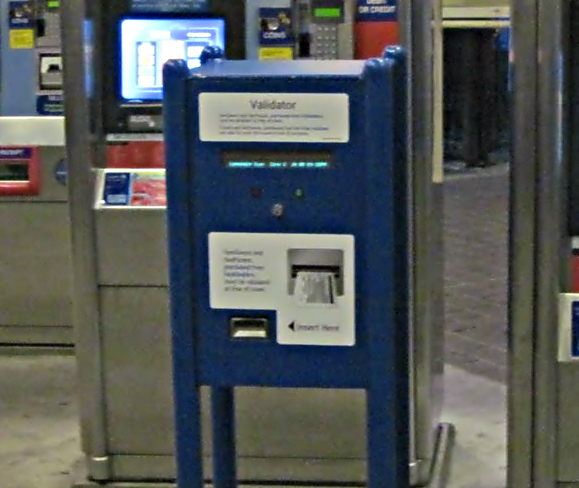
\includegraphics[width=90mm]{tv5tvm.jpg}
\caption{Old ticket validator}
\end{figure}

We then created a ticket ``cooking'' procedure: a ticket is first encoded with a forged date and time, and with a Sign Number that doesn't match the one used at Burrard station (10002). This \emph{half-cooked} ticket is then scanned in the old Burrard station validator machines, which change the Sign Number field and write the new data onto the ticket. This produces a magnetic ticket encoded using the exact same physical parameters as an authentic ticket. This \emph{fully-cooked} ticket can then be scanned at all Translink ticket readers including busses, skytrain, canada line and seabus, and will appear genuine.

We calculated that the maximum expiry date is Dec 31, 1999 $+ 2^{14}-1$ days, which is November 7, 2044 (a Monday). If the maximum expiry time is added to this value, it becomes November 8, 2044, at 5:30PM (after adding 239 * 6 minutes). We created several prototype tickets which expire at this time, referred to as \emph{millennium tickets} due to their timeless nature. We found that every Translink machine is vulnerable to these millennium tickets.

\section{Sign Number}
Once we determined that the first stored data field represented some kind of machine ID, we began searching for a database which matched the values we had seen in order to augment our analysis tools. We checked all publicly-available data on Translink's domains including the Google Maps transit schedule data, but the machine ID numbers weren't used in that context.

Eventually we found a vulnerability in the Canadian Auto Workers Union (CAW Local 111) website \cite{caw111} which allowed us to access the bus operator scheduling information. 

\newpage

\lstset{breaklines=true}
\lstset{showspaces=false,showstringspaces=false}
\lstset{basicstyle=\ttfamily\scriptsize}
\begin{figure}[ht!]
\begin{lstlisting}

C M B C PRINT DATE: 13/02/13 OPERATORS PADDLE PAGE: 1 of 3 DATABASE: 13APR Mon-Fri LINE GROUP: 027 BLOCK NO. 1 EFF: Apr 15, 2013
---------------------------------------------------------------
BTC DEPOT: 604 293-4604 CONTROL: 778 593-5524
---------------------------------------------------------------
LINE: 026 EB1 (WHEEL CHAIR ACCESSIBLE) (BIKE RACK EQUIPPED) SIGN #168 SIGN: "26 JOYCE STN"; Start 29TH AVE STN (BAY #3) R/E 29TH AVE R/EARLES ST L/KINGSWAY R/SCHOOL AVE R/RUPERT ST C/KERR ST L/ROSEMONT DR R/BUTLER ST L/MAQUINNA DR R/CHAMPLAIN CR L/MATHESON CR R/ARBOR AVE L/BOUNDARY RD L/E 49 AVE R/TYNE ST L/E 45 AVE R/JOYCE ST L/VANNESS R/JOYCE STN
LINE: 026 WB1 (WHEEL CHAIR ACCESSIBLE) SIGN #169 (BIKE RACK EQUIPPED) SIGN: "26 29TH AVE STN"; Start JOYCE STN (BAY #3) R/JOYCE ST L/E 45TH AVE R/TYNE ST L/E 49TH AVE R/FRONTENAC ST L/HURST AVE R/BOUNDARY RD R/ARBOR AVE L/MATHESON CR R/CHAMPLAIN CR L/MAQUINNA DR R/BUTLER ST L/ROSEMONT DR R/KERR ST Conti RUPERT ST L/KINGSWAY R/EARLES ST L/E 29TH AVE L/29TH AVE STN
LINE: 027 NB1 (WHEEL CHAIR ACCESSIBLE) SIGN #175 (BIKE RACK EQUIPPED) SIGN: "27 KOOTENAY LOOP"; Start JOYCE STN (BAY #2) L/JOYCE ST L/WELLINGTON AVE R/RUPERT ST C/BUS LANE, C/RUPERT ST R/ADANAC ST L/BOUNDARY RD L/E HASTINGS ST R/KOOTENAY LOOP
LINE: 027 NB3 (WHEEL CHAIR ACCESSIBLE) SIGN #175 (BIKE RACK EQUIPPED) SIGN: "27 KOOTENAY LOOP"; Start KINGSAY & JOYCE Via KINGSWAY R/JOYCE ST L/VANNESS AVE(BAY #2) R/JOYCE STN LOOP L/JOYCE ST L/WELLINGTON AVE R/RUPERT ST C/BUS LANE C/RUPERT ST R/ADANAC ST L/BOUNDARY RD L/E HASTINGS ST R/KOOTENAY LOOP
\end{lstlisting}
\caption{Raw route information from \texttt{caw111.com}}
\end{figure}

\lstset{basicstyle=\ttfamily\small}



The ``SIGN \#'' referenced in these documents matched the machine ID values we had decoded. We wrote a tool to collect all the schedule sheets including those from previous years, which provided us a database of every bus route's Sign Number used over the last several years. We then scanned tickets at various Skytrain stations and Canada Line stations and determined that these routes use incrementing Sign Numbers.

\begin{figure}[ht!]
\centering
\begin{lstlisting}[language=C]
{1521, "N10 BRIGHOUSE STN"},
{1522, "N10 BRIGHOUSE STN VIA YVR NIGHTBUS"},
{1523, "49 LANGARA-49 STN"},
{1527, "BRIDGEPORT STN"},
{1529, "311 BRIDGEPORT STATION"},
{1530, "301 BRIGHOUSE STN"},
{1531, "3 MAIN-MARINE STN"},
{1542, "N10 DOWNTOWN NIGHTBUS"},
{1543, "9 COMMERCIAL - BROADWAY"},
{1545, "100 MARPOLE VIA TRAPP"},
{1546, "10 TO DAVIE"},
\end{lstlisting}
\caption{Extracted bus route Sign Numbers}
\end{figure}

Skytrain Expo Line stations use Sign Numbers 10001 - 10020, representing Waterfront, Burrard, Granville, Stadium, Main St, Broadway, Nanaimo, 29th Ave, Joyce, Patterson, Metrotown, Royal Oak, Edmonds, 22nd St, New West, Columbia, Scott Road, Gateway, Surrey Central, and King George. Skytrain Millennium Line stations use Sign Numbers 10031 - 10043, representing VCC/Clark, Commercial, Renfrew, Rupert, Gilmore, Brentwood, Holdom, Sperling, Lake City Way, Production Way, Lougheed, Braid, and Sapperton. Canada Line stations use Sign Numbers 50 - 65, representing Waterfront, VCC, Yaletown, Olympic Village, Broadway, King Edward, Oakridge, Langara, Marine Drive, Bridgeport, Templeton, Sea Island Centre, YVR-Airport, Aberdeen, Landsdowne, and Richmond-Brighouse. Tickets purchased directly from one of the YVR stations incur a \$5 surcharge, and these tickets are given the Sign Number 73. The Seabus terminals use Sign Number 10090. The full list of Sign Numbers is available at \cite{bussesh}.

Using this database, we can determine the bus route or transit station where any ticket was purchased or scanned. 

\section{Skytrain}
Skytrain ticket checking is performed visually, by security agents who verify the date and time printed on the back of a Translink ticket. We determined two methods of forging this verification procedure.

The first method entails repeatedly overwriting a used ticket with the bit sequence of an unused Faresaver. When an unused Faresaver is first scanned, the expiry date and time are printed on the back. When the ticket is scanned a second time, the machine knows that the ticket has been validated, and must already have had text printed on it. We repeatedly caused this text to be printed, which creates an unreadable blur. We found that Translink security guards routinely encounter tickets with blurred text due to ongoing mechanical faults in the ticket vending machine printers, and simply accept the tickets as genuine.


As a second attack, we analyzed the dot-matrix writing technique used on the ticket vending machines and created a TrueType font (TTF) which replicates this writing style.

\begin{figure}[ht!]
\centering

\includegraphics[width=120mm]{font.png}
\caption{Translink ticket font \cite{ttf}}
\end{figure}

A ticket can thus be forged by printing the desired expiry time on a blank ticket, or a piece of paper that has been printed and cut like a ticket. Considering the price of a 3-zone ticket is currently \$5.50, this is a plausible forgery technique.

\section{Conclusion}
I managed to create fully spoofed millennium tickets. I spent \$75 in hardware costs to obtain a credit card writing machine, and didn't spend any money on tickets for analysis.

I performed this research alone, and didn't base my analysis on any prior research. I was carrying my U-Pass at all times when I was testing the forged tickets, so that I wouldn't be in violation of fare regulations.


\begin{thebibliography}{9}

\bibitem{debut}
  Translink,
  \emph{New electronic fareboxes debut on Vancouver buses and trolleys this Monday},
  \url{http://www.translink.ca/en/About-Us/Media/2001/November/New-electronic-fareboxes-debut-on-Vancouver-buses-and-trolleys-this-Monday.aspx}.
  November 16, 2001.
  
\bibitem{ubc}
  Timothy D. Kinisky, Michael D.G. Hewitt, Derek Kwei, Colleen Qin, 
  \emph{Analysis and Design of a Smart Card Transit Security System}.
  UBC Engineering,
  2005.

\bibitem{tyner}
  Tyner Corp.,
  \emph{MSR206 Magnetic Stripe Card Reader/Writer (High \& Low Coercivity)}.
  Apr. 06, 2005.
  
\bibitem{caw111}
  Canadian Auto Workers Local 111, 
  \url{http://www.caw111.com/}.
  
\bibitem{bussesh}
  git://github.com/qartis/translink/busses.h,
  \url{https://github.com/qartis/translink/blob/master/busses.h}.

  
\bibitem{ttf}
  git://github.com/qartis/translink/translink.ttf,
  \url{https://github.com/qartis/translink/blob/master/translink.ttf}.

\end{thebibliography}
\end{document}

